% Verwendete Pakete und andere Definitionen:
\documentclass[ %
english, % Sprache
12pt, % Standardschriftgröße
a4paper, % Papierformat
titlepage, % Titelseite aktivieren
twoside=on, % Zweiseitiges Layout
numbers=noenddot, % Überschriftennummerierung ohne Punkt am Ende
bibliography=totoc, % Literaturverzeichnis im Inhaltsverzeichnis aufführen
chapterprefix=true, % Kapitel steht vor \chapter-Befehl
open=right % Kapitel auf ungerader Seitenzahl beginnen
]{scrreprt} % Dokumenteigenschaften
\usepackage[utf8]{inputenc} % wie Editoreingaben umwandeln (Umlaute, Sonderzeichen, ...)
\usepackage{float}
\usepackage{mathtools}
\usepackage{ragged2e} %Für text Blocksatz
\usepackage{babel} % Sprachpakete
\usepackage[T1]{fontenc} % Encoder für Font
\usepackage{amsmath,amsthm,amssymb} % Zum Einbinden von Formeln
\usepackage{amssymb} % Zum Einbinden von Symbolen
\usepackage{color} % Für Farben
\usepackage{wrapfig} %To wrap text around figures
\usepackage{afterpage} %Make stuff appear on next page
\usepackage{calc} % Rechenoperationen innerhalb Befehlsdefinitionen
\usepackage[ %
automark, % Automatische Labelsetzung für Kopfzeile
headsepline % Trennstrich zwischen Kopfzeile und Text
]{scrpage2} % Für eigene Kopf- und Fußzeile 
\usepackage{graphicx} % Zum Einfügen von Grafiken
\usepackage{natbib}
\usepackage{graphics}
\usepackage{mathptmx} % Standardschrift ist Times New Roman (auch in Formeln)
\usepackage[rightcaption]{sidecap} % Überschrift neben Bild
\usepackage[ %
format=plain, % Beschriftung ist gewöhnlicher Absatz
justification=justified, % Blocksatz
font=small, % Schriftgröße
labelfont=bf, % Fettes Label
labelsep=colon, % Doppelpunkt als Trenner
figurename=Figure, % Labelname für Bild
tablename=Table % Labelname für Tabelle
]{caption} % Für Bildunterschriften
\usepackage[hypcap=true,subrefformat=simple]{subcaption} % Mehrere Bilder nebeneinander mit Unterschrift
%\usepackage{titlesec} % Überschrifen formatieren
\usepackage[separate-uncertainty]{siunitx} % Für Einheiten
\usepackage{booktabs} % Tabellen besser formatieren können, für ExcelToLatex Makro
\usepackage{tikz,pgfplots} %For graphs and plots
\usepgfplotslibrary{groupplots}
\pgfplotsset{compat=1.6}

\usetikzlibrary{positioning} 
%\usepackage{multirow} % Tabellen besser formatieren können, für ExcelToLatex Makro
%\usepackage{bigstrut} % Tabellen besser formatieren können, für ExcelToLatex Makro
%\usepackage{enumitem} % Für spezielle Aufzählungen
\usepackage[version=3]{mhchem} % Für chemische Formeln

\usepackage[top=4.5cm,bottom=6cm,left=2.75cm,right=3cm,footskip=1cm]{geometry} % Layout
\usepackage[ %
bookmarks=true, % Zeige Lesezeichenleiste
pdftitle={Distinct propagation of brain activity patterns for aversive emotions with and without cognitive regulation}, % Titel
pdfauthor={Sascha Frölich}, % Autor
colorlinks=true, % Umrandete (Box) oder farbige Links
linkcolor=black, % interne Linkfarbe
urlcolor=blue, % Farbe von URL links
citecolor=black % Farbe für Zitierungslinks
]{hyperref} % Links in Pdf - Paket muss als letztes geladen werden!!!
%
% Format von Bildreferenz: \ref{} --> 1.1(a), \subref{} --> (a)
\renewcommand\thesubfigure{(\alph{subfigure})}
%
% Schriftart setzen (Einheitlich Times New Roman) + Überschriften fett:
\setkomafont{disposition}{\bfseries}
%
% Anzahl Ebenen im Inhaltsverzeichnis
\setcounter{tocdepth}{2}
%
% Überschriften formatieren:
%\titlespacing*{\section}{0pt}{*3}{*1.5} % Abstand vor und nach Überschrift
%\titleformat{\section}[hang]{\Large\bfseries}{\makebox[1.5cm][l]{\thesection}}{0pt}{}
%\titleformat{\subsection}[hang]{\large\bfseries}{\makebox[1.5cm][l]{\thesubsection}}{0pt}{}
%\titleformat{\subsubsection}[hang]{\normalsize\bfseries}{\makebox[1cm][l]{\thesubsubsection}}{0pt}{}
%
% Befehl für Referenzen auf Formeln, mit \eref{...} aufrufen
\newcommand{\eref}[1]{Eq.~\eqref{#1}}
%
% Befehl für Referenzen auf Bilder, mit \fref{...} aufrufen
\newcommand{\fref}[1]{Fig.~(\ref{#1})}
%
% Befehl für Referenzen auf Tabellen, mit \tref{...} aufrufen
\newcommand{\tref}[1]{Tab.~\ref{#1}}
%
% Befehl für Referenz  auf einen Abschnitt, mit \sref{...} aufrufen
\newcommand{\sref}[1]{Sec.~\ref{#1}}

\setlength\parskip{\baselineskip}
\usepackage[section]{placeins} % Place floats in the section they are in
%
% Zusammenfügung aller Teildokumente:
\begin{document}
\pgfmathdeclarefunction{gauss}{3}{%
  \pgfmathparse{1/(sqrt(2*pi*#3))*exp(-((#1-#2)^2)/(2*#3))}%
}

	\pagenumbering{Roman} % Erste Seiten haben römische Seitenzahlen
	\begin{titlepage}
	\vspace*{0.5cm}
	\begin{center}
		\begin{minipage}{5.5cm} %statt 5.5
			\centering
			
\includegraphics[width=4.5cm]{images/logos/TUD} %statt 5
		\end{minipage}
	\end{center}
	\vspace*{0cm}
	\begin{center}
		\begin{minipage}{5.5cm}
			\centering
			\textsc{Technische \\ Universit\"{a}t \\ Dresden}
		\end{minipage}
		\hfill
		\begin{minipage}{3.5cm}
			\centering
			\textsc{}
		\end{minipage}
		\hfill
		\begin{minipage}{5cm}
			\centering
			\textsc{Lehrstuhl f\"{u}r Neuroimaging}
		\end{minipage}
	\end{center}
	\vspace*{1cm}
	\begin{center}
		\Huge \textbf{Different formulations of the same problem}\\[1.5cm]
		\large \textbf{}\\[2.25cm]
		\large Sascha Fr\"{o}lich\\[0.25cm]
		\large Dresden, 2019 \\[0.5cm]
	\end{center}
\end{titlepage}
 % Titelseite
	\cleardoublepage
	%\begin{center}
	%\textit{To my Father.}
	%\end{center}
	\begingroup
	  	\renewcommand*{\chapterpagestyle}{empty}
	  	\pagestyle{empty} % Keine Seitenzahl für Inhaltsverzeichnis
	  	\tableofcontents % Inhaltsverzeichnis
	  	\cleardoublepage
	\endgroup
	\pagestyle{scrheadings} % Seitenstil setzen
	\setcounter{page}{1} % Titelseite und Inhaltsverzeichnis sollen nicht mitgezählt werden
	\pagenumbering{arabic} % Ab hier arabische Seitenzahlen
	%
	\chapter{Different formulations of the same problem with examples}
\label{sec:ELBO}

AS MANY PICTURES AS POSSIBLE!!!

DO NOT FORGET COIN EXAMPLE

\section{Introduction}
\noindent For the remainder of this overview, we will always return to the specific example of determining the fairness of a coin, where the latent variable $z$ is the \textit{true} fairness of a coin, where $z=0.5$ indicates that the coin will show heads exactly half of the time. \\

\noindent $z$ - latent variables \\
\noindent $\theta$ - model parameters (i.e. latent variables. Therefore $\theta \in z$ (see below)) \\
\noindent $y$ - data, observation \\
\noindent $m$ - model (categorical variable) \\

\subsection{Notation}

\noindent Here I want to address a first point of confusion. Often we see different notations for the same thing, such as $q(z,\phi)$ and $q_{\phi}(z)$ for one and the same thing, and $p(y|m)$, or $p(y)$ for another thing. Sometimes we even see stuff like

\begin{equation}
p(x|\theta) = \frac{exp(-\frac{(x-\mu)^2}{2\sigma^2})}{\sqrt{2\pi \sigma^2}} = p(\theta|x),
\end{equation}

therefore

\begin{equation}
p(x|\theta) = p(\theta|x).
\end{equation}

\noindent What does all of this mean? Let's go through this step by step.

\subsubsection{\underline{$q(z,\phi)$ vs $q_{\phi}(z)$}}
In most of the literature, and throughout this treatment, $z$ is a latent (i.e. hidden) variable which is to be inferred, while $\theta$, $\phi$ often stands for the set of parameters of a model. In the case where our model is represented by a Gaussian distribution, these are be the mean and variance $\theta=\{\mu,\sigma\}$. So $\theta$ describes the parameters of the Gaussian distribution, while the distribution itself is a function of $z$ (EXPLANATORY PICTURE?). Therefore, the notation $p_\theta(z)$ might be useful as it tells us we are dealing with a distribution over $z$, parametrized by $\theta$, while notations such as $\Phi = \{ p_{\theta 1}, p_{\theta 2}, ... \}$ make clear we are dealing with a number of normal distributions, all with their own parameters. In inference problems, however, parameters themselves often have to be inferred themselves and can therefore be treated as latent variables. This is why we will always use notations like $p(z,\theta)$. At this point, we might as well include the latent variables $\theta$ into the set of other latent variables $z$.

\subsubsection{\underline{$p(y|m)$ vs $p(y)$}}

In the beginning this was very confusing to me, especially identities such as $p(x|theta) = p(\theta|x)$ as described before.  $p(\cdot |m)$ is to be understood as <<under a given model>>.


\emph{MEANING OF THE WORD <<MODEL>>}

\subsection{Energies and logarithms}

\noindent While we do not want to be bothered with the details for now, the main point to note that throughout the literature, the term \textit{energy} is used when talking about the logarithms of probability distributions $p(x)$. This comes from the fact that in statistical physics, the distribution of many interesting quantities of ensembles of particles (like the velocity distribution of air molecules in a box at a given temperature) can be described as $p(x) = \alpha \cdot e^{-E(x)}$, where $E(x)$ is the energy, given the quantity of interest $x$ (velocity, say). Beyond this rather simple analogy, there is not much more to it. The interested reader may refer to the \sref{sec:EnergiesAndLogs} for a more profound treatment of the physical origins of this.


\section{Variational Inference}

Given a specific model $m$, we have a probability distribution $p(x|m)$. For example, say $m = \mathcal{N}(\mu,\Sigma)$ (i.e. a normal distribution), then \\

\begin{align*}
p(x|m) = \frac{exp(-\frac{(x-\mu)^2}{2\sigma^2})}{\sqrt{2\pi \sigma^2}}.
\end{align*}

On its own, a probability distribution does not have any specific meaning when dealing with Bayesian inference, as in Bayesian inference a probability distribution can have many different meanings. When I talk about a \textit{model}, however, I generally think about the joint probability distribution $p(y,z)$ of observed data $y$ and hidden variables $z$, which consists of the \textit{likelihood} $p(y|z)$ and the \textit{prior} $p(z)$, which, in turn, are probability distributions of their own.

\noindent Given a specific model m, and parameters $\theta$ (e.g. $\theta = \{\mu, \sigma\}$), the \textit{model evidence} is 

$p(y|m) = \int p(y|\theta)p(\theta|m)d\theta$. 

\noindent The model evidence, or \textbf{marginal likelihood}, is the integral over all parameter values of the model. This can then be used to compare different models to select the best one, which is the one maximizing $p(y|m)$. [Murphy, page 158].  In the Free Energy formulation, the negative of the model evidence is interpreted as the \textbf{surprise}, which needs to be minimized (as the model evidence is to be maximized).\\

\noindent Once we did a number of different observations $y = \{y_1, y_2, ...\}$, we can compute the \textit{likelihood} $p(\theta|y,m)$ of a given model, which is a scalar value given a specific model and its parameters. The likelihood tells us (in arbitrary units), how \textit{likely} the parameters of our model are. For different parameters of the same model, and the same observations, we therefore get a function wrt to the parameters $\theta$, which is the \textit{likelihood function}:

\begin{equation}
p(\theta | y,m).
\end{equation}

This is a function of the model parameters $\theta$, and given a model and data we can choose those parameters which maximize that function which would then return the parameters which make observing the given data most likely (given the model). This is called \textit{Maximum Likelihood Estimation}. Now assume we want to perform Bayesian inference on the fairness of a coin. We are interested in the hidden variable $z$, which is equal to the actual fairness of the coin (probability of showing heads), and should be $0.5$ in the fairest case. After a number of coin flips $y={1,0,1,1...} (1=\text{heads})$, the Bayesian inference problem looks as follows: \\

\begin{equation}
p(z|y)= \frac{p(y|z)p(z)}{p(y)} \propto p(y|z)p(z),
\end{equation}

\noindent where we omit the $m$ for the model (for simplicity). We could write $p(y|z,m)p(z,m)$, but in a practical example this would just mean something like <<the likelihood and the prior, given that we know what form they are supposed to take>>. In a practical setting, the condition on $m$ is met just by knowing what forms those distributions are to take, which you need to know in order to be able to actually compute something with them, obviously. Confusingly enough, $p(y|z)$ is also called the likelihood and must not be confused with the likelihood function above. While the nominator is basically our <<view of the world>> (i.e.) our model, and is strongly dependent on our beliefs, the denominator $p(y)$ gives the <<true>> probability of the observed data (or \textit{evidence}) and is generally not accessible to us. However this shall not further concern us, as it is just a normalizing constant and does not influence the inference process, as most inference processes boil down to finding maxima of functions and are quite independent of their actual value. $p(z)$ is the \textit{prior} over our hidden variable $z$ and constitutes our prior believe of what value $z$ is likely to take on. In the unbiased case, we might choose $p(z)$ to be a Beta distribution around $0.5$. The \textit{likelihood} $p(y|z)$ is the Bernoulli distribution (for one observed coin flip) or, equivalently, the binomial distribution for a number n of coin flips. Our goal is to find out $p(z|y)$ (Bishop page 463). But this is not always easily doable (WHY). Therefore, we define an \textit{approximate posterior} $q(z)$, which we will try to bring as close to $p(z|y)$ as possible. We want thus to minimize $D_{KL}(q(z)||p(z|y))$. This is still pretty complicated, as evaluating $p(z|y)=\frac{p(y|z)p(z)}{p(y)}$ would require the (unknown) normalization constant $p(y)$. Therefore we try to minimize the following instead\footnote{$D_{KL}(f(x)||g(x))$ is the \textit{Kullback-Leibler} divergence. It is a similarity measure between probability distributions and is defined as $D_{KL}(f(x)||g(x))= \int f(x)\log\frac{f(x)}{g(x)} dx$. It is probably a good idea to remember this definition by heart. Note how it cannot generally be used as a similarity measure between \textit{functions}, as $\log\frac{f(x)}{g(x)}$ will then not be guaranteed to be positive.}:

\begin{equation}
D_{KL}(q(z)||p(z,y)) = \int q(z)\log \frac{q(z)}{p(z,y)} = F[q(z)]
\label{eq:FE}
\end{equation}[Murphy, page 734], which is the \textit{variational free energy}. We take a second to let that sink in: \textbf{The Variational Free Energy is the distance between the approximate posterior and the (auxiliary) joint distribution}\footnote{The term \textit{Free Energy} comes first and foremost from the fact that it looks very similar to the concept of Free Energy in statistical physics. For a short introduction to the concept of Free Energy in statistical physics, see \sref{sec:FE_app}.}. Reordering that equation:

\begin{equation}
\int q(z)\log \frac{q(z)}{p(z,y)} dz= \int q(z)\left[ \log \frac{q(z)}{p(z|y)} - \log p(y) \right]dz,
\end{equation}

\noindent and thus\footnote{Using $\int dz q(z)\log p(y) = p(y)$, as $q(z)$ is a probability distribution.}

\begin{equation}
D_{KL}(q(z)||p(z,y)) = D_{KL}(q(z)||p(z|y)) - \ln p(y).
\end{equation}

\noindent Therefore, \textbf{minimizing the variational free energy by tweaking $q(z)$ minimizes the distance between the approximate posterior and the true posterior}. This is true, as changing $q(z)$ does not have an effect on $\ln p(y)$ and can therefore be considered a constant in this context. \\

\noindent As $D_{KL}$ is always greater than zero, the negative of the Free Energy is a lower bound of the model evidence $p(y)$ (sometimes $p(y|m)$). This lower bound is sometimes called the \textit{evidence lower bound}, or \textit{ELBO}.

\noindent Rewriting \eref{eq:FE}, we find the following:

\begin{equation}
 F[q(z)] = - \left<\ln p(y,z) -\ln q(z) \right>_{q(z)},
\end{equation}

\noindent which reformulates the free energy in terms of an energy term and an entropy term. FEW WORDS ON ENTROPY TERM

\section{ToDo}

1) The unrestricted Free Energy Principle is Bayesian Inference [Samuel Gershman: What does the free energy principle tell us about the brain?]

2) Bayesian Central Limit Theorem: justification for Gaussian assumption [Gershman]

3) Laplace approx: Linearize Free Energy around the posterior mode, as Free Energy is usually not tractable [Gershman]

4) Predictive Coding as an aspect of FEP [Gershman]

5) Active Inference: Minimization of expected Free Energy

\chapter{Hamilton's Principle}

As stated in the previous chapters, during Bayesian Inference, we want to find the true posterior distribution $p(z|y)$. For reasons of simplicity, we assume that all probability distributions are Gaussian distributions. This is called the \textit{Laplace approximation}. In this case, all we are really interested in is the mean of the distribution $p(z|y)$, ignoring the variance for a moment. The mean $\mu$ of $p(z|y)$ is the coordinate where the distribution assumes its maximum. Numerically, this maximum can be reached via a gradient ascent scheme:

\begin{align*}
\dot{\mu_g} = \frac{d}{dz} \ln p(z|y),
\end{align*}
where the subscript $g$ stands for <<guessed>>, as the true mean is always at the true mode of the energy $\ln p$, while we are trying to approach that true mean via gradient ascent of our guessed mean $\mu_g$. Importantly,  $\dot{\mu_g}$ does not stand for the <<natural>> evolution of $\mu_g$ with time, but for the change we need to apply to it in order to make it closer to the mode of the energy. \\

\noindent The above case is true for static systems, but what if $p(z|y)$ changes over time? Answer:

\begin{align*}
\dot{\mu_g} = D\mu_g + \frac{d}{dz} \ln p(z|y),
\end{align*}

where now $D\mu$ is the <<natural>> time-evolution of the mean. This corrects the guessed mean such that it accounts for the distance to the actual mean as well as for their natural time-evolution.
\begin{center}
\begin{figure}
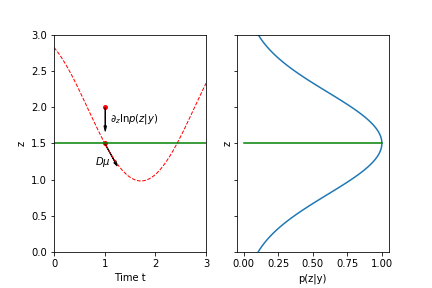
\includegraphics[scale=0.7]{images/FE_ex_4}
\caption{The true mode of the probability distribution $p(z|y)$ is at $z=1.5$ (green line), while the <<guessed>> mean is at $z=2$. The dashed red line describes the time evolution of the mode of the probability distribution, which is described by the differential operator $D$ acting on $\mu$. The correction $\dot{mu}$ to be applied to the guessed mean is then $\frac{d}{dz} \ln p(z|y) + D\mu$.}
\end{figure}
\end{center}
[Friston \& Kiebel, Predictive Coding under the free energy principle; Friston: Hierarchical models in the brain].
	\chapter{State-Space Models and Hierarchical Dynamics}
\label{sec:SSM}

BLablabla
	\chapter{Bayesian Inference With Probability Distributions}
\label{sec:Prob_Distros}

\section{MAP Inference}
A classic MAP inference scheme will look like this:

\begin{align}
\text{Posterior} \propto \text{Likelihood}\cdot \text{Prior}.
\label{eq:MAP}
\end{align}
In order to obtain a probability distribution as posterior, it will then be necessary to normalize the resulting Posterior to integrate to 1. In sequential update schemes, the posterior to work with would then be

\begin{align}
\frac{\text{Posterior}}{Z},
\label{eq:Normalization}
\end{align}
where $Z$ is a normalizing constant. The posterior is also called the agent's \textit{belief}

\subsection{Product of Gaussian PDFs}

As gaussian distributions are priors to themselves, there may arise situations in which the chosen likelihood function as well as the prior distribution are gaussians. The product of two gaussian distributions
\begin{align*}
\mathcal{N}(x;\mu_1,\sigma_1 ^2) \\
\mathcal{N}(x;\mu_2,\sigma_2 ^2)
\end{align*}

will then be a gaussian function, but not a distribution, as it is not normalized. 

\begin{align}
& \mathcal{N}(x;\mu_1,\sigma_1 ^2) \cdot \mathcal{N}(x;\mu_1,\sigma_1 ^2) \\
&= \mathcal{N}(x;\frac{\mu_1 \sigma_2 ^2 +\mu_2 \sigma_1 ^2}{\sigma_1 ^2\cdot \sigma_2 ^2},\frac{\sigma_1 ^2\cdot \sigma_2 ^2}{\sigma_1 ^2+ \sigma_2 ^2})\cdot e^{-\frac{C}{2\frac{\sigma_1^2 \sigma_2^2}{\sigma_1^2 + \sigma_2^2}}}, \\
C & =\frac{\sigma_1^2 \sigma_2^2}{(\sigma_1^2 + \sigma_2^2)^2}\left[ (\mu_1 -\mu_2)^2 +\ln(2\pi(\sigma_1^2 + \sigma_2^2)) \right],
\label{eq:normal_product}
\end{align}
with normakization constant $Z=\exp{\left(-\frac{C}{2\frac{\sigma_1^2 \sigma_2^2}{\sigma_1^2 + \sigma_2^2}}\right) }$
In Bayesian Inference, we are however always interested in probability distributions. Therefore, we need to normalize the resulting gaussian function, which returns

\begin{align}
\text{Posterior} = \mathcal{N}(x;\frac{\mu_1 \sigma_2 ^2 +\mu_2 \sigma_1 ^2}{\sigma_1 ^2\cdot \sigma_2 ^2},\frac{\sigma_1 ^2\cdot \sigma_2 ^2}{\sigma_1 ^2+ \sigma_2 ^2}).
\label{eq:Posterior}
\end{align}

\subsection{Maximum Likelihood Estimate}

\section{Example: On a Boat}
You are on a boat. You are trying to figure out your direction of travel. Directly in front of you is a lighthouse. You know that the lighthouse is more or less at 25 degrees from north, but you are not 100$\%$ sure about its exact location. You perform a series of 10 measurements with a noisy measurement device, which indicates that the lighthouse is about 65 degrees from north.

\begin{tikzpicture}
\begin{axis}[
  no markers, 
  domain=0:90, 
  samples=300,
  ymin=0,
  axis lines*=left, 
  xlabel=$\theta$,
  every axis y label/.style={at=(current axis.above origin),anchor=south},
  every axis x label/.style={at=(current axis.right of origin),anchor=west},
  height=5cm, 
  width=12cm,
  ytick=\empty,
  enlargelimits=false, 
  clip=false, 
  axis on top,
  grid = major,
  hide y axis,
  xtick distance=10
  ]

 \addplot [very thick,blue] {gauss(x, 25, 25)};
  \addplot [very thick,red!50!black] {gauss(x, 65, 25)};
   \addplot [very thick,orange] {gauss(x, 45, 12.5)};

\draw[dashed] (axis cs:25,0) -- (axis cs:25,0.08);
\draw[dashed] (axis cs:65,0) -- (axis cs:65,0.08);

\node[below] at (axis cs:25, 0)  {$\mu_1$}; 
\node[below] at (axis cs:65, 0)  {$\mu_2$}; 

\node[below] at (axis cs:0, -0.01)  {North}; 
\node[below] at (axis cs:45, -0.01)  {Northeast}; 
\node[below] at (axis cs:90, -0.01)  {East}; 

\node[text=blue] at (axis cs:10,0.07) {Prior};
\node[text=red] at (axis cs:80,0.09) {Measurements = Likelihood};
\node[text=orange] at (axis cs:55,0.11) {Posterior};

\node[text=black] at (axis cs:0,-0.05) {Figure ???};

\end{axis}
\end{tikzpicture}

Bayesian Inference according to \eqref{eq:MAP} and \eqref{eq:Normalization} suggests a posterior as given in the picture. It might at first be an intuitive solution: Your inferred posterior is exactly in the middle between prior and likelihood if both have the same precision. From the figure, and from \eqref{eq:Posterior} it is however clear, that the variance of the resulting posterior is independent of the distance from the likelihood to the prior. Furthermore, the posterior's variance will always be smaller than the variance of either likelihood or prior. This is a not reasonable. If my prior indicates one direction, and the likelihood a completely other direction, it might be reasonable to infer the middle, but it does not make sense to be even more certain about the midway direction than about both prior and likelihood. \\

This is a misinterpretation of Bayesian Inference. In Bayesian inference, the latent variables which one wishes to infer \textit{are taken to be probability distributions}. This is in contrast to classical physics, where model parameters are taken to be fixed, while our observations of them are noisy. In Bayesian Inference, much like in quantum mechanics, we make the important distinction to think of latent variables as probability distributions. Our measurements of those variables are however fixed, which is equivalent to the collapse of the wave function in QM. The narrowing of the posterior as seen in the figure above only describes our increased certainty about the mean of the probability distribution which itself \textit{is} the latent variable $\theta$. The variance of $\theta$ would be subject to another inference process. \\

As an aside, I want to point out an interesting property of the Free Energy formulation. As can be seen from \eqref{eq:normal_product}, the normalization constant $Z$ will become very small if Likelihood and Prior are very far apart. Interestingly, the Free Energy takes on the form [Schwöbel et al]

\begin{align}
F = -\ln Z -\sum \ln Z.
\end{align} 

Thus, small normalization constants produce large free energy, which is supposed to be minimized.

\section{Example: German Tank Problem}

\section{Example: A needle on an infinite grid}
Blablabla Stochastikübung normal und mit "Bayes"
	\chapter{Appendix}

\section{Free Energy}
\label{sec:FE_app}
This article will try to give an intuitive review of the Free Energy as it is defined in statistical physics. We will see that Free Energy is a measure of a system's capacity to do work and that its minimization is a statistical necessity for a closed system. For the sake of clarity, I will use examples and interpretations which are not physically rigorous but help to develop a good understanding of the matter.

The toy example we are looking at is a two-state system which consists of ten "particles" which can take on two discrete energy values $E_0 = 0 J$ and $E_1 = 1 J$. A real-world analogon might be a collection electrons inside a magnetic field. Electrons whose spins are aligned parallel to the field correspond to particles in the lower energy level, while electrons with spins antiparallel to the field lines reside on the higher energy level (see Fig 1).

\begin{figure}
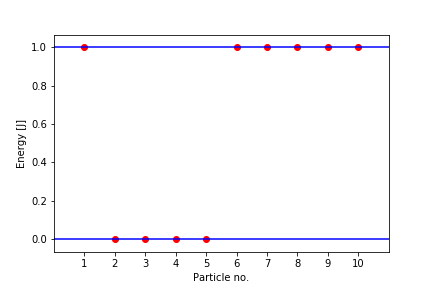
\includegraphics[scale=0.5]{images/FE_ex_1}
\caption{A two-level system with energy $E = 6J$}
\end{figure}

We will now consider one such system whose total energy is known to be $6J$. This means that six of its particles reside on the upper energy level while four particles occupy the lower level. One such possible system is shown in Figure 1. The committed reader may now pause for a second and consider for themselves if the displayed system appears to be in equilibrium or not. The (hopefully intuitive) answer is no. While we did not yet consider what "equilibrium" actually means, it may feel intuitive that in the given case, it means that the excited particles at energy $1J$ and the particles at energy $0J$ are somehow evenly distributed and do not clump together in one small region of the system.

In our case of of a 10-particle system with energy of $6J$, the number of possible microstates is 

$$\Omega_0(E = 6J) = {10\choose 6} = \frac{10!}{6!\cdot 4!} = 210.$$

In order to understand the main point of this article, we will apply a little trick whose use will become apparent later. We will split the system of ten particles into two compartments of five particles, the left of which we will call System A, while the other is System B (Fig. 2).

\begin{figure}
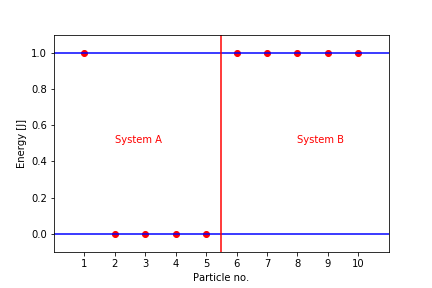
\includegraphics[scale=0.5]{images/FE_ex_2}
\caption{We separate the total System into two subsystems.}
\end{figure}

Next, we will go on to find the \textit{most likely} energy configurations of systems $A$ and $B$ such that their total energy $E = E_A + E_B$ equals $6 J$. We will find that the most probable energy configuration is the homogeneous state $E_A = E_B = 3J$ and that this state is reached by minimization of free energy or, equivalently, maximization of entropy.

\subsection{Finding the Probability for a given Energy of System A}

The question we are now trying to anser is:
\\
\\
For a system composed of two systems $A$ and $B$ as above, with total energy $E$, how likely is System $A$ to assume a specific energy level $E_A$?

In order to do this, we have to rely on one of the great postulates of statistical physics which we will accept as given (see Bibliography):
\\
\\
POSTULATE: In the equilibrium state, all possible microstates of a system are equally likely.
\\
\\
This postulate is also known as the \textit{The Fundamental Assumption of Statistical Mechanics}.
Using this postulate, our original question can be cast into mathematical form for the probability of System $A$ to have energy $E_A$. This is equal to the ratio of microstates that realize that energy to all other possible microstates that would result in a total energy of $E = 6J$:

$$W(E_A) \equiv (\text{Probability of System A assuming energy level }E_A) = \frac{\Omega_A(E_A)\cdot \Omega_B(E_B = E -E_A)}{\Omega_0(E)} \text{     (Eq. 1)}.$$

As this formula might feel intimidating for the mathematical layperson, I will go through it step by step:
$\Omega(E_A)$ is the number of microstates of System A that would realize a specific energy $E_A$. For our example (Figure 1), that energy corresponds to one particle in System A sitting on the upper energy level, thus $E_A = 1J$. For a total of 5 particles in System A, this is true for 5 different microstates, therefore $\Omega(E_A) = 5$. As we started with a known total energy $E = E_A + E_B$ (in our example 6J), requiring $E_A$ to be equal to $1J$ determines System B's energy $E_B = 5J$. The number of microstates that realize this is $\Omega(E_B = 5J) = 1$, as all particles in System B have to be in the upper state. The total number of different configurations such that $E_A$ is assumed by System A and $E_B$ by System B is therefore the product of the number of different microstates $\Omega_A(E_A)$ and $\Omega_B(E_B)$. The probability that any of these configurations is assumed is then equal to the ratio of that product with the number of all other possible microstates $\Omega_0(E)$ such that the total energy is $E$. In our case of 10 particles, six of which have to be in the upper energy level, that number is 210, as seen above. Therefore, the probability of finding our energy configuration in Figure 1 for a system at equilibrium is

$$W(E_A = 1J) = \frac{\Omega_A(E_A = 1 J)\cdot \Omega_B(E_B = 5J)}{\Omega_0(E = 6J)} = \frac{1\cdot 1}{210} \approx 0.005.$$

\subsection{Finding the most likely Energy for System A}

We are now interested in the most likely energy configuration for Systems $A$ and $B$ in the equilibrium state. The general idea is to find the value $\bar{E_A}$, for which $W(E_A)$ assumes a maximum value. This value can be found by setting the derivative of the probability function $W(E_A)$ to zero.

$$\frac{d}{d E_A} \ln (W(E_A)) = 0$$

The fact that we are deriving $\ln W(E_A)$ instead of $W(E_A)$ may not concern us here. The reason this is commonly done in statistical physics is that the maximum of the function $W(E_A)$ is at the same position as the maximum of the function $\ln W(E_A)$, while the latter is mathematically easier to deal with than the former. 

The energy $\bar{E_A}$ which maximizes $W(E_A)$ is then found to be the energy at which the energy is homogeneously dsitributed across the system:

$$\frac{\bar{E_A}}{f_A} = \frac{\bar{E_B}}{f_B} (Eq. 2),$$

where $f_i$ denotes the number of degrees of freedom of system i. In our example, the number of degrees of freedom is equal to the number of particles. What this means is that the most likely state a system at equilibrium will find itself in is a state of homogeneous energy distribution. This can be deduced from a purely statistical way of reasoning: The system at equilibrium can be found in each microstate with the same probability. The energy configuration the system will mos likely be found in is therefore the configuration which has the highest number of possible microstates. That energy configuration is however exactly the homogeneous case, where all imagined subsystem contain the same energy. More concretely, for our example:

$E_A = 1J \rightarrow \Omega_A(E_A)\cdot \Omega_B(E_B) = 5$

$E_A = 2J \rightarrow \Omega_A(E_A)\cdot \Omega_B(E_B) = 50$

$E_A = 3J \rightarrow \Omega_A(E_A)\cdot \Omega_B(E_B) = 100$

$E_A = 4J \rightarrow \Omega_A(E_A)\cdot \Omega_B(E_B) = 50$

$E_A = 5J \rightarrow \Omega_A(E_A)\cdot \Omega_B(E_B) = 5$


\begin{figure}
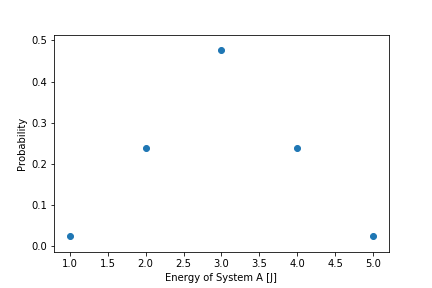
\includegraphics[scale=0.5]{images/FE_ex_3}
\caption{The probability for System A to have half of the total energy is highest.}
\end{figure}

The entropy is defined as 

$$S = k_B \ln \Omega(E).$$

Furthermore, entropy is an extensive property, i.e. the entropy of an ensemble of subsystems is the sum of the entropies of the single systems. 


Furthermore, entropy is an extensive property, i.e. the entropy of an ensemble of subsystems is the sum of the entropies of the individual systems:

$$\Omega(E) = \Omega_A(E_A)\cdot \Omega_A(E_A) \rightarrow S = k_B \ln \Omega(E) = k_B \ln \left( \Omega_A(E_A)\cdot \Omega_A(E_A) \right) \rightarrow S = S_A + S_B$$

Via the relations between the energy configurations of the subsystems and the number of microstates which would realize such configuration, it is easily seen that the entropy in this example is maximized by the homogeneous distribution of energies where $S_A = S_B$.

\subsection{Free Energy}

The (Helmholtz) Free Energy $F$ is defined as

$$F = E -TS,$$

where $E$ is the internal energy of the system and $T$ the (fixed) temperature of the system (equivalent to the system being in contact with a heat bath). As we have seen before, a closed system will always strive towards the equilibrium state which is equivalent to maximization of entropy. Given that $T$ is considered fixed, maximization of entropy thus corresponds to minimaztion of the free energy $F$. Note that the assumption of a given temperature $T$ is important here as otherwise $E$ and $T$ might be related via $$ \frac{1}{T} = \frac{dS}{dE}.$$


\subsection{Physical interpretation and work}

The above example was rather mathematical without much emphasis on physical interpretation. However, the concept of minimization of free energy $F$ does also have a very elegant physical interpretation.

As the minimum value of $F$ is reached when energy is homogeneously distributed across the system, a non-minimal value of $F$ is equivalent to local energy inhomogeneities. That is to say that the energy density varies from one point in the system to another. These changes in density can be described as energy gradients. Much like an electric potential is the necessary driver for flow of electric current, those energy gradients may create energy flows which, again, strive to reduce overall inhomogeneity. These energy flows can be harnessed to perform work. It is for this reason that free energy is generally considered as a measure of the energy with which a system can perform work. A system with high internal energy will not be able to perform work if that energy is completely homogeneously distributed.


\subsection{Temperature}

A homogeneous distribution of energy has as a direct consequence that the system at hand has the same temperature everywhere. This can easily be seen considering the equipartition theorem which relates the mean energy of a system in equilibrium with its temperature. For an ideal gas, the mean energy per atom is:

$$\bar{E} = \frac{3}{2}k_BT$$



\subsection{Conclusion}

Given the example considerations we can summarize the following:

1) The increase of entropy (and thus the decrease of free energy) is a statistical necessity. It describes a closed system's tendency to approach an equilibrium distribution with a homogeneous distribution of energy.

2) Free Energy is a measure of how far the system is from its equilibrium state. It is also a measure of the energy a system can harness to perform work.

2) This minimization of free energy $F$ can be interpreted on a physically level, as follows. Because a non-maximum value of the entropy (and thus non-minimal value of the Free Energy) corresponds to an inhomogeneous distribution of energy, minimization of $F$ is equivalent to saying that the system contains energy gradients with spatial extension larger than any single constituent (particle, say) of the system. These energy gradients are natural drivers of energy exchange, thus energy flow. This flow of energy can be harnessed to do work and thus drive motion. Internal energy alone does not give any information of a system's capacity to do work, while the distribution of energy within the system (i.e. its free energy) does.

4) By the above train of reasoning, the minimization of free energy corresponds to a well-known fact from biology: namely that every (living) system strives for homeostasis, i.e. internal equilibrium.


\subsection{Bibliography}

Torsten Fließbach: Statistische Physik IV


\subsection{Suggested Further Reading}

[1] E.T. Jaynes: Gibbs vs Boltzmann Entropies, American Journal of Physics \textbf{33}, 391 (1965).

Link: https://aapt.scitation.org/doi/pdf/10.1119/1.1971557?class=pdf

[2] E.T. Jaynes: The Gibbs Paradox. Link: https://bayes.wustl.edu/etj/articles/gibbs.paradox.pdf

\section{Energies and Logarithms}
\label{sec:EnergiesAndLogs}

Quite often we are dealing with logarithms of probability distributions and call them energies. In some cases, energies are minimized, in others they are maximized [Friston \& Kiebel: Predictive Coding under the Free Energy Principle].  I want to clarify where those ideas come from, and what they mean. \\

\noindent  In physics, energies and probability distributions are finely intertwined. Imagine the following problem (adapted from the Feynman lectures on Physics): Given the density of the atmosphere at ground level, how dense are the air molecules at a given altitude $h$? The only reason why the density of the air is higher at ground level than at higher altitudes is due to the earth's gravitational force, such that at ground level you have to withstand the pressure created by all the air molecules above you. Those molecules are pulled down by the earth's gravitational field. Analogously, you might as well just talk about an air molecule's potential energy: The higher up, the more potential energy. It turns out that the air density $n$ density at any height $h$ is exactly a function of the potential energy at that height:

\begin{align*}
n = \alpha e^{-\beta E_{pot}},
\end{align*}
with some constants $\alpha, \beta$. \\

\noindent Now consider this question: Given a box full of air with temperature $T$, what is the probability for particle to have velocity $v$? The answer is

\begin{align*}
f(u)du = const \cdot e^{-\beta E_{kin}(u)}du
\end{align*}
for a velocity between $u$ and $u+du$. Thus, the \textit{probability distribution} (or more accurately \textit{probability density function}) of the velocities is

\begin{align*}
f(u) = const \cdot e^{-\beta E_{kin}(u)}.
\end{align*}

It turns out that basically any probability density function which describes the distribution of a quantity of interest in a thermodynamic setting with conservative forces can be written in terms of the corresponding kinetic and potential energies, as above. [Feynman, Statistical Physics] \\

\noindent Given a probability distribution of the form $p(x) = e^{-E(x)}$ (omitting constants), one can easily see that $E(x) = -\ln p(x)$. As in Bayesian Inference, we are dealing a lot with the logarithms of probability distributions, it has become convenient to refer to them as energies. It is however important to note that those \textit{energies} do not usually have a physical interpretation, or any other meaningful interpretation. The expression comes purely from the analogy with statistical physics.

\section{Identities}
\begin{align}
FE &= D_{KL}(q(z)||p(z|y)) - \ln p(y) \\
&= -ELBO \\
& = - \left<\ln p(y,z) -\ln q(z) \right>_{q(z)}.
\end{align}

\section{Ergodicity}
Probabilities do not exist. They only exist in repetition experiments. Blablabla
	\chapter{ToDo}
\label{sec:todo}

Include fun stuff \\
Berkson's paradox \\
Poisson Distro \\
\end{document}